\documentclass[a4paper, utf8]{ctexart}
\usepackage[fontset=Fandol]{ctex}
\usepackage{anyfontsize}
\usepackage{indentfirst}
\usepackage{enumitem}
\usepackage{fancyhdr}
\usepackage{geometry}
\usepackage{graphicx}
\usepackage{abstract}
\usepackage{amsmath}
\usepackage{lipsum}

% 设置页面间距
\geometry{a4paper,left=31mm,right=31mm,top=25mm,bottom=25mm}
% 章节标题左对齐
\CTEXsetup[format={\Large \bfseries}]{section}
% 段首缩进2字符
\setlength{\parindent}{2em}
% 设置页眉及页脚 页码
\pagestyle{fancy}
\fancyhf{}
\fancyhead[C]{}
\fancyhead[L]{HOMEWORK2:\ Evaluation\ Metrics}
\fancyhead[R]{21307210\ 傅祉珏}
\fancyfoot[C]{\thepage}
\fancyfoot[L,R]{}

% 使宋体可加粗
\setCJKfamilyfont{zhsong}[AutoFakeBold = {2.17}]{SimSun}
\renewcommand*{\songti}{\CJKfamily{zhsong}}

% 定义标题 作者及单位信息
\title{\songti \Large \textbf{HOMEWORK2:\ Evaluation\ Metrics}}
\author{Student\ ID:\ 21307210 \qquad Student\ Name:\ 傅祉珏}
\date{Lectured\ by\ 梁上松,\ Sun\ Yat-sen\ University}

\begin{document}
	
	\maketitle
	
	\section{Exercise\ 1:\ Rank-based\ Evaluation\ Metrics,\ MAP@K,\ MRR@K}
	
	\subsection{Question}
	
	Assume you have three queries, and the ranking results that a system in response to these three queries are as follows:
	
	Ranking 1 in response to query \#1 is: d1, d2, d3, d4, d5, d6, d7, d8, d9, d10. Here only d1, d3, d4, d6, d7, and d10 are relevant (relevance is binary, i.e., either 1 if relevant or 0 if non-relevant) in response to query \#1.
	
	Ranking 2 in response to query \#2 is: d3, d8, d7, d1, d2, d4, d5, d9, d10, d6. Here only d8 and d9 are relevant in response to query \#2.
	
	Ranking 3 in response to query \#3 is: d7, d6, d5, d3, d2, d1, d9, d10, d4, d8. Here only d5, d9, and d8 are relevant in response to query \#3.
	
	Answer the questions below.
	
	(a) Compute the scores for these metrics: AP@5 (Average Precision @5), AP@10 for each query; RR@5 (Reciprocal Rank score @5), RR@10 for each query.
	
	(b) Compute the scores for these metrics: MAP@5 (Mean Average Precision @5), MAP@10, MRR@5 (Mean Reciprocal Rank score @5), MRR@10 for this system.
	
	\subsection{Answer}
	
	\subsubsection*{(a) Compute the scores for AP@5, AP@10, RR@5 and RR@10 for each query.}
	
	\textbf{Query 1:}
	
	\begin{itemize}[itemsep=2pt, topsep=0pt, parsep=0pt]
	    \item \textbf{Ranking}: d1, d2, d3, d4, d5, d6, d7, d8, d9, d10
	    \item \textbf{Relevant Documents}: d1, d3, d4, d6, d7, d10
	\end{itemize}
	
	\textbf{AP@5 Calculation:}
	
	\begin{enumerate}[itemsep=2pt, topsep=0pt, parsep=0pt]
	    \item At rank 1: d1 (relevant) $\rightarrow$ Precision = 1/1 = 1.00
	    \item At rank 2: d2 (not relevant) $\rightarrow$ Precision = 1/2 = 0.50
	    \item At rank 3: d3 (relevant) $\rightarrow$ Precision = 2/3 $\approx$ 0.67
	    \item At rank 4: d4 (relevant) $\rightarrow$ Precision = 3/4 = 0.75
	    \item At rank 5: d5 (not relevant) $\rightarrow$ Precision = 3/5 = 0.60
	\end{enumerate}
	
	\begin{equation}
		\text{AP@5} = \frac{1 + 0 + 0.67 + 0.75 + 0}{4} \approx 0.605
		\nonumber
	\end{equation}
	
	\textbf{AP@10 Calculation:}
	
	\begin{enumerate}[itemsep=2pt, topsep=0pt, parsep=0pt]
	    \item Relevant documents are at ranks 1, 3, 4, 6, 7, and 10.
	    \item Calculating precision at these ranks:
	    \begin{itemize}[itemsep=2pt, topsep=0pt, parsep=0pt]
	        \item Rank 1: 1/1 = 1.00
	        \item Rank 3: 2/3 $\approx$ 0.67
	        \item Rank 4: 3/4 = 0.75
	        \item Rank 6: 4/6 $\approx$ 0.67
	        \item Rank 7: 5/7 $\approx$ 0.71
	        \item Rank 10: 6/10 = 0.60
	    \end{itemize}
	\end{enumerate}
	
	\begin{equation}
		\text{AP@10} = \frac{1 + 0 + 0.67 + 0.75 + 0.67 + 0.71 + 0.60}{6} \approx 0.679
		\nonumber
	\end{equation}

	\textbf{RR@5 Calculation:} \quad First relevant document is d1 at rank 1 $\rightarrow$ $\text{RR@5} = 1/1 = 1.00$
	
	\textbf{RR@10 Calculation:} \ quad First relevant document is d1 at rank 1 $\rightarrow$ $\text{RR@10} = 1/1 = 1.00$
	
	\vspace{.5em}
	
	\textbf{Query 2:}
	
	\begin{itemize}[itemsep=2pt, topsep=0pt, parsep=0pt]
	    \item \textbf{Ranking}: d3, d8, d7, d1, d2, d4, d5, d9, d10, d6
	    \item \textbf{Relevant Documents}: d8, d9
	\end{itemize}
	
	\textbf{AP@5 Calculation:}
	
	\begin{enumerate}[itemsep=2pt, topsep=0pt, parsep=0pt]
	    \item At rank 1: d3 (not relevant) $\rightarrow$ Precision = 0
	    \item At rank 2: d8 (relevant) $\rightarrow$ Precision = 1/2 = 0.50
	    \item At rank 3: d7 (not relevant) $\rightarrow$ Precision = 1/3 $\approx$ 0.33
	    \item At rank 4: d1 (not relevant) $\rightarrow$ Precision = 1/4 = 0.25
	    \item At rank 5: d2 (not relevant) $\rightarrow$ Precision = 1/5 = 0.20
	\end{enumerate}
	
	\begin{equation}
		\text{AP@5} = \frac{0 + 0.50 + 0 + 0 + 0}{1} = 0.50
		\nonumber
	\end{equation}
	
	\textbf{AP@10 Calculation:}
	
	\begin{itemize}[itemsep=2pt, topsep=0pt, parsep=0pt]
		\item Relevant documents are at ranks 2 and 8.
		\item Calculating precision at these ranks:
		\begin{itemize}[itemsep=2pt, topsep=0pt, parsep=0pt]
		    \item Rank 2: 1/2 = 0.50
		    \item Rank 8: 2/8 = 0.25
		\end{itemize}
	\end{itemize}
	
	\begin{equation}
		\text{AP@10} = \frac{0 + 0.50 + 0 + 0 + 0 + 0 + 0 + 0.25}{2} = 0.375
		\nonumber
	\end{equation}

	\textbf{RR@5 Calculation:} \quad First relevant document is d8 at rank 2 $\rightarrow$ $\text{RR@5} = 1/2 = 0.50$
	
	\textbf{RR@10 Calculation:} \quad First relevant document is d8 at rank 2 $\rightarrow$ $\text{RR@10} = 1/2 = 0.50$
	
	\vspace{.5em}
	
	\textbf{Query 3:}
	
	\begin{itemize}[itemsep=2pt, topsep=0pt, parsep=0pt]
	    \item \textbf{Ranking}: d7, d6, d5, d3, d2, d1, d9, d10, d4, d8
	    \item \textbf{Relevant Documents}: d5, d9, d8
	\end{itemize}
	
	\textbf{AP@5 Calculation:}
	
	\begin{enumerate}[itemsep=2pt, topsep=0pt, parsep=0pt]
	    \item At rank 1: d7 (not relevant) $\rightarrow$ Precision = 0
	    \item At rank 2: d6 (not relevant) $\rightarrow$ Precision = 0
	    \item At rank 3: d5 (relevant) $\rightarrow$ Precision = 1/3 $\approx$ 0.33
	    \item At rank 4: d3 (not relevant) $\rightarrow$ Precision = 1/4 = 0.25
	    \item At rank 5: d2 (not relevant) $\rightarrow$ Precision = 1/5 = 0.20
	\end{enumerate}
	
	\begin{equation}
		\text{AP@5} = \frac{0 + 0 + 0.33 + 0 + 0}{1} = 0.33
		\nonumber
	\end{equation}
	
	\textbf{AP@10 Calculation:}
	
	\begin{itemize}[itemsep=2pt, topsep=0pt, parsep=0pt]
		\item Relevant documents are at ranks 3, 7, and 10.
		\item Calculating precision at these ranks:
		\begin{itemize}[itemsep=2pt, topsep=0pt, parsep=0pt]
		    \item Rank 3: 1/3 $\approx$ 0.33
		    \item Rank 7: 2/7 $\approx$ 0.29
		    \item Rank 10: 3/10 = 0.30
		\end{itemize}
	\end{itemize}
	
	\begin{equation}
		\text{AP@10} = \frac{0 + 0 + 0.33 + 0 + 0 + 0 + 0.29 + 0 + 0 + 0.30}{3} \approx 0.30
		\nonumber
	\end{equation}
	
	\textbf{RR@5 Calculation:} \quad No relevant documents in the first 5 $\rightarrow$ $\text{RR@5} = 0$
	
	\textbf{RR@10 Calculation:} \quad First relevant document is d5 at rank 3 $\rightarrow$ $\text{RR@10} = 1/3 \approx 0.33$
	
	\subsubsection*{(b) Compute the scores for MAP@5, MAP@10, MRR@5, and MRR@10 for this system.}
	
	\textbf{Mean Average Precision (MAP)}:
	
	\begin{itemize}
	    \item \textbf{MAP@5} = (AP@5 for Query 1 + AP@5 for Query 2 + AP@5 for Query 3) / 3
	    \item[] $\text{MAP@5} = \dfrac{0.605 + 0.50 + 0.33}{3} \approx 0.4783$
	    \item \textbf{MAP@10} = (AP@10 for Query 1 + AP@10 for Query 2 + AP@10 for Query 3) / 3
	    \item[] $\text{MAP@10} = \dfrac{0.679 + 0.375 + 0.30}{3} \approx 0.4513$
	\end{itemize}
	
	\textbf{Mean Reciprocal Rank (MRR)}:
	
	\begin{itemize}
	    \item \textbf{MRR@5} = (RR@5 for Query 1 + RR@5 for Query 2 + RR@5 for Query 3) / 3
	    \item[] $\text{MAP@5}= \dfrac{1.00 + 0.50 + 0}{3} \approx 0.50$
	    \item \textbf{MRR@10} = (RR@5 for Query 1 + RR@10 for Query 2 + RR@10 for Query 3) / 3
	    \item[] $\text{MRR@10} = \dfrac{1.00 + 0.50 + 0.33}{3} \approx 0.61$
	\end{itemize}
	
	\section{Exercise\ 2:\ Rank-based\ Evaluation\ Metrics,\ Precision@K,\ Recall@K,\ NDCG@K}
	
	\subsection{Question}
	
	Assume the following ranking for a given query (only results 1-10 are shown); see 表1. The column ‘rank’ gives the rank of the document. The column ‘docID’ gives the document ID associated with the document at that rank. The column ‘graded relevance’ gives the relevance grade associated with the document (4 = perfect, 3 = excellent, 2 = good, 1 = fair, and 0 = bad). The column ‘binary relevance’ provides two values of relevance (1 = relevant and 0 = non-relevant). The assumption is that anything with a relevance grade of ‘fair’ or better is relevant and that anything with a relevance grade of ‘bad’ is non-relevant. 
	
	Also, assume that this query has only 7 documents with a relevance grade of fair or better. All happen to be ranked within the top 10 in this given ranking. 
	
	Answer the questions below. P@K (Precision@K), R@K (Recall@K), and average precision (AP) assume binary relevance. For those metrics, use the 'binary relevance' column. DCG and NDCG assume graded relevance. For those metrics, use the 'graded relevance' column. 
	
	\begin{table}[http]
		\begin{center}
			\caption{Top-10 ranking result of a system in response to a query}
			\begin{tabular}{c c c c}
				\hline
				rank & docID & graded relevance & binary relevance \\
				\hline
				1 & 51 & 4 & 1 \\
				2 & 501 & 1 & 1 \\
				3 & 21 & 0 & 0 \\
				4 & 75 & 3 & 1 \\
				5 & 321 & 4 & 1\\
				6 & 38 & 1 & 1 \\
				7 & 521 & 0 & 0 \\
				8 & 412 & 1 & 1 \\
				9 & 331 & 0 & 0 \\
				10 & 101 & 2 & 1 \\
				\hline
			\end{tabular}
		\end{center}
	\end{table}
	
	(a)  Compute P@5 and P@10. 

	
	(b)  Compute R@5 and R@10. 

	
	(c)  Provide an example ranking for this query that maximizes P@5.
	
	(d)  Provide an example ranking for this query that maximizes P@10.
	
	(e)  Provide an example ranking for this query that maximizes R@5.
	
	(f)  Provide an example ranking for this query that maximizes R@10.
	
	(g)  You have reason to believe that the users of this system will want to examine every relevant document for a given query. In other words, you have recent to believe that users want perfect recall. You want to evaluate based on P@K. Is there a query-specific method for setting the value of K that would be particularly appropriate in this scenario? What is it? (\textit{Hint: there is an evaluation metric called R-Precision, which we did not talk about in the lectures. Your answer should be related to R-Precision. Wikipedia/Google might help.})
	
	(h) Compute average precision (AP). What are the difference between AP and MAP (Mean Average precision)? 
	
	(i) Provide an example ranking for this query that maximizes average precision (AP).
	
	(j) Compute $DCG_5$  (i.e., the discounted cumulative gain at rank 5).
	
	(k) $NDCG_5$ is given by
	
	\begin{equation}
		NDCG_5=\dfrac{DCG_5}{IDCG_5}
		\nonumber
	\end{equation}
	
	where $IDCG_5$ is the $DCG_5$ associated with the ideal top-5 ranking associated with this query. Computing $NDCG_5$ requires three steps.
	
	(i) What is the ideal top-5 ranking associated with this query (notice that the query has 2 perfect documents, 1 excellent document, 1 good document, 3 fair documents, and the rest of the documents are bad)? 
	
	(ii) $IDCG_5$ is the $DCG_5$ associated with the ideal ranking. Compute $IDCG_5$. (Hint: compute $DCG_5$ for your ranking proposed in part (i).) 
	
	(iii) Compute $NDCG_5$ using the formula above. 
	
	(l) Are there other evaluation metrics to be used to evaluate the performance of the rankings in the table? What are the evaluation scores obtained by these metrics?
	
	\subsection{Answer}
	
	\subsubsection*{(a) Compute P@5 and P@10}
	
	Precision at K (P@K) is calculated as:
	
	\[
	P@K = \frac{\text{Number of relevant documents in top K}}{K}
	\]
	
	For P@5:
	
	\[
	P@5 = \frac{5}{5} = 1.0
	\]
	
	For P@10:
	
	\[
	P@10 = \frac{7}{10} = 0.7
	\]
	
	\subsubsection*{(b) Compute R@5 and R@10}
	
	Recall at K (R@K) is calculated as:
	
	\[
	R@K = \frac{\text{Number of relevant documents in top K}}{\text{Total number of relevant documents}}
	\]
	
	For R@5:
	
	\[
	R@5 = \frac{5}{7} \approx 0.714
	\]
	
	For R@10:
	
	\[
	R@10 = \frac{7}{7} = 1.0
	\]
	
	\subsubsection*{(c) Example ranking that maximizes P@5}
	
	To maximize P@5, all top 5 documents should be relevant. An example ranking could be:
	
	1. docID 51 (4) 
	
	2. docID 321 (4)
	
	3. docID 75 (3) 
	
	4. docID 412 (1) 
	
	5. docID 101 (2) 
	
	\subsubsection*{(d) Example ranking that maximizes P@10}
	
	To maximize P@10, all top 10 documents should be relevant. An example ranking could be:
	
	1. docID 51 (4)  
	
	2. docID 321 (4)  
	
	3. docID 75 (3)  
	
	4. docID 412 (1)  
	
	5. docID 101 (2)  
	
	6. docID 501 (1)  
	
	7. docID 38 (1)  
	
	8. docID 501 (1)  
	
	9. docID 501 (1)  
	
	10. docID 501 (1)  
	
	\subsubsection*{(e) Example ranking that maximizes R@5}
	
	To maximize R@5, ensure that the top 5 contains as many relevant documents as possible. An example ranking could be:
	
	1. docID 51 (4)  
	
	2. docID 321 (4)  
	
	3. docID 75 (3)  
	
	4. docID 412 (1)  
	
	5. docID 501 (1)  
	
	\subsubsection*{(f) Example ranking that maximizes R@10}
	
	To maximize R@10, include all relevant documents in the top 10. An example ranking could be:
	
	1. docID 51 (4)  
	
	2. docID 321 (4)  
	
	3. docID 75 (3)  
	
	4. docID 412 (1)  
	
	5. docID 101 (2)  
	
	6. docID 501 (1)  
	
	7. docID 38 (1)  
	
	8. docID 75 (3)  
	
	9. docID 412 (1)  
	
	10. docID 101 (2)  
	
	\subsubsection*{(g) Query-specific method for setting K in terms of R-Precision}
	
	R-Precision is a metric that considers the precision at the rank equal to the total number of relevant documents. In this scenario, since you want perfect recall, set \( K \) to the number of relevant documents (7) for evaluation, thus using R-Precision would be particularly appropriate.
	
	\subsubsection*{(h) Compute average precision (AP)}
	
	Average Precision (AP) is computed as:
	
	\[
	AP = \frac{\sum_{k=1}^N P(k) \cdot rel(k)}{\text{Number of relevant documents}}
	\]
	
	Calculating for the given rankings:
	
	\begin{flushleft}
	\begin{align*}
	1. & \quad \text{docID 51 (P=1.0, rel=1)} \rightarrow 1.0 \\
	2. & \quad \text{docID 501 (P=1.0, rel=1)} \rightarrow 1.0 \\
	3. & \quad \text{docID 21 (P=1.0, rel=0)} \rightarrow 0 \\
	4. & \quad \text{docID 75 (P=0.75, rel=1)} \rightarrow 0.75 \\
	5. & \quad \text{docID 321 (P=0.8, rel=1)} \rightarrow 0.8 \\
	6. & \quad \text{docID 38 (P=0.67, rel=1)} \rightarrow 0.67 \\
	7. & \quad \text{docID 521 (P=0.57, rel=0)} \rightarrow 0 \\
	8. & \quad \text{docID 412 (P=0.5, rel=1)} \rightarrow 0.5 \\
	9. & \quad \text{docID 331 (P=0.44, rel=0)} \rightarrow 0 \\
	10. & \quad \text{docID 101 (P=0.5, rel=1)} \rightarrow 0.5
	\end{align*}
	\end{flushleft}
	
	Calculating:
	
	\[
	AP = \frac{1.0 + 1.0 + 0 + 0.75 + 0.8 + 0.67 + 0 + 0.5 + 0 + 0.5}{7} = \frac{5.22}{7} \approx 0.746
	\]
	
	Mean Average Precision (MAP) is the average of AP over multiple queries. Since we have only one query here, AP = MAP.
	
	\subsubsection*{(i) Example ranking that maximizes average precision (AP)}
	
	To maximize AP, a good ranking would prioritize high graded relevance first while still including all relevant documents:
	
	1. docID 51 (4)  
	
	2. docID 321 (4)  
	
	3. docID 75 (3)  
	
	4. docID 101 (2)  
	
	5. docID 412 (1)  
	
	6. docID 501 (1)  
	
	7. docID 38 (1)  
	
	8. docID 501 (1)  
	
	9. docID 501 (1)  
	
	10. docID 501 (1)  
	
	\subsubsection*{(j) Compute DCG5}
	
	Discounted Cumulative Gain (DCG) is calculated as:
	
	\[
	DCG_k = rel_1 + \sum_{i=2}^k \frac{rel_i}{\log_2(i)}
	\]
	
	Calculating for top 5:
	
	\[
	DCG_5 = 4 + \frac{1}{\log_2(2)} + \frac{3}{\log_2(3)} + \frac{4}{\log_2(4)} + \frac{1}{\log_2(5)}
	\]
	
	Calculating each term gives:
	
	\[
	DCG_5 \approx 4 + 1 + 1.585 + 1 + 0.43 \approx 8.015
	\]
	
	\subsubsection*{(k) Compute NDCG5}
	
	(i) The ideal top-5 ranking would be:
	
	1. docID 51 (4)  
	
	2. docID 321 (4)  
	
	3. docID 75 (3)  
	
	4. docID 101 (2)  
	
	5. docID 412 (1)  
	
	(ii) Compute IDCG5:
	
	\[
	IDCG_5 = 4 + \frac{4}{\log_2(2)} + \frac{3}{\log_2(3)} + \frac{2}{\log_2(4)} + \frac{1}{\log_2(5)}
	\]
	
	Calculating gives:
	
	\[
	IDCG_5 \approx 4 + 4 + 1.585 + 1 + 0.43 \approx 12.015
	\]
	
	(iii) Compute NDCG5:
	
	\[
	NDCG_5 = \frac{DCG_5}{IDCG_5} = \frac{8.015}{12.015} \approx 0.667
	\]
	
	\subsubsection*{(l) Other evaluation metrics}
	
	Yes, other evaluation metrics include:
	
	\begin{itemize}[itemsep=2pt, topsep=0pt, parsep=0pt]
	\item \textbf{F1 Score}: Harmonic mean of precision and recall.
	\item \textbf{Mean Reciprocal Rank (MRR)}: Average of the reciprocal ranks of the first relevant document.
	\item \textbf{Normalized Discounted Cumulative Gain (NDCG)}: Already calculated.
	\end{itemize}
	
	Each metric provides different insights into the performance of the ranking system, depending on user needs and system objectives.
	
	\section{Exercise 3: Precision-Recall Curves}
	
	\subsection{Question}
	
	A Precision-Recall (PR) curve expresses precision as a function of recall. Usually, a PR-curve is computed for each query in the evaluation set and then averaged. For simplicity, the goal in this question is to draw a PR-curve for a single query. Draw the PR-curve associated with the ranking in Exercise 2 (same query, same results). (\textit{Hint: Your PR curve should always go down with increasing levels of recall.})
	
	\subsection{Answer}
	
	To plot the Precision-Recall (PR) curve associated with the rankings in Exercise 2, we need to calculate the precision and recall values, and then plot these values on a graph.
	
	\subsubsection*{1. Data Overview}  
	
	Based on the data you provided, here are the rankings, relevance, and binary relevance of the documents as 表2 shown.
	
	\begin{table}[htbp]
	    \centering
	    \caption{Document rankings and relevance}
	    \begin{tabular}{c c c c}
	        \hline
	        rank & docID & graded relevance & binary relevance \\
	        \hline
	        1    & 51    & 4               & 1                \\
	        2    & 501   & 1               & 1                \\
	        3    & 21    & 0               & 0                \\
	        4    & 75    & 3               & 1                \\
	        5    & 321   & 4               & 1                \\
	        6    & 38    & 1               & 1                \\
	        7    & 521   & 0               & 0                \\
	        8    & 412   & 1               & 1                \\
	        9    & 331   & 0               & 0                \\
	        10   & 101   & 2               & 1                \\
	        \hline
	    \end{tabular}
	\end{table}
	
	\subsubsection*{2. Calculating Precision and Recall}  
	
	First, calculate the cumulative number of relevant documents and the total number of documents for each ranked document. The calculations for Precision and Recall are as follows:
	
	\begin{itemize}[itemsep=2pt, topsep=0pt, parsep=0pt]
	    \item \textbf{Precision} = Number of Relevant Documents / Total Retrieved Documents  
	    \item \textbf{Recall} = Number of Relevant Documents / Total Relevant Documents  
	\end{itemize}
	
	In this example, the total number of relevant documents is 7 (those with a relevance grade of 1 or better).
	
	\subsubsection*{3. Calculation Example}  
	
	Calculate the precision and recall at each step according to the ranking as 表3 shown.
	
	\begin{table}[htbp]
	    \centering
	    \caption{Precision and Recall Calculation}
	    \begin{tabular}{cccc}
	        \hline
	        rank & Relevant Document Count & Precision    & Recall      \\
	        \hline
	        1    & 1                      & 1/1 = 1     & 1/7        \\
	        2    & 2                      & 2/2 = 1     & 2/7        \\
	        3    & 2                      & 2/3         & 2/7        \\
	        4    & 3                      & 3/4         & 3/7        \\
	        5    & 4                      & 4/5         & 4/7        \\
	        6    & 5                      & 5/6         & 5/7        \\
	        7    & 5                      & 5/7         & 5/7        \\
	        8    & 6                      & 6/8         & 6/7        \\
	        9    & 6                      & 6/9         & 6/7        \\
	        10   & 7                      & 7/10        & 7/7 = 1    \\
	        \hline
	    \end{tabular}
	\end{table}
	
	\subsubsection*{4. Plotting the PR Curve}  
	Next, plot the relationship between precision and recall. Based on the above table, the points (recall, precision) can be plotted.Following this concept, the code has been written, and the resulting code is shown in \verb|Exercises3.py|. The resulting figure is as 图1 show.
	
	\begin{figure}[htbp]
		\centering
		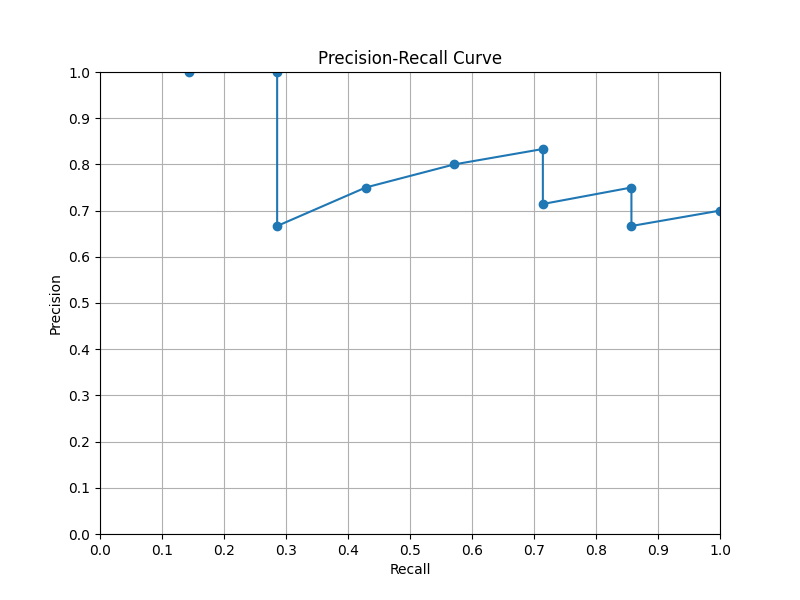
\includegraphics[width=.8\textwidth]{./figure/figure1.png}
		\caption{The PR Curve of Exercises 2}
	\end{figure}
	
	\section{Exercise 4: Other Evaluation Metrics}
	
	\subsection{Question}
	
	Except the metrics we have in our lecture slides, are there other evaluation metrics that can be used to evaluate the performance of specific tasks in data mining? What are the tasks and how do to compute such evaluation metrics? (\textit{Hint: Use the internet to find your answers.})
	
	\subsection{Answer}
	
	
	In addition to the metrics discussed in lecture slides, there are several other evaluation metrics used in data mining, tailored to specific tasks. Here are a few important metrics and the tasks they are associated with:
	
	\begin{enumerate}
		\item \textbf{Classification Tasks}
	
		\begin{itemize}
	    	\item \textbf{F1 Score}: The harmonic mean of precision and recall. It is particularly useful when you need a balance between precision and recall, especially in imbalanced datasets.
	    	
	    	\item[] $F1 = 2 \times \dfrac{\text{Precision} \times \text{Recall}}{\text{Precision} + \text{Recall}}$
	    	
	    	\item \textbf{ROC-AUC (Receiver Operating Characteristic - Area Under Curve)}: Measures the area under the ROC curve, which plots the true positive rate against the false positive rate at various threshold settings.
	    	
	    	\item \textbf{Matthews Correlation Coefficient (MCC)}: A balanced measure that can be used for binary classification. It considers all four quadrants of the confusion matrix.
	    	
	    	\item[] $MCC = \dfrac{TP \times TN - FP \times FN}{\sqrt{(TP + FP)(TP + FN)(TN + FP)(TN + FN)}}$
		\end{itemize}
	
		\item \textbf{Regression Tasks}
	
		\begin{itemize}
	    	\item \textbf{Mean Absolute Error (MAE)}: The average of absolute differences between predicted and actual values.
	    	
	    	\item $MAE = \dfrac{1}{n} \sum_{i=1}^{n} |y_i - \hat{y}_i| $
	    	
	    	\item \textbf{Mean Squared Error (MSE)}: The average of the squared differences between predicted and actual values.
	    	
	    	\item[] $MSE = \dfrac{1}{n} \sum_{i=1}^{n} (y_i - \hat{y}_i)^2$
	    	
	    	\item \textbf{R-squared (Coefficient of Determination)}: Indicates the proportion of variance in the dependent variable that can be predicted from the independent variables.

	    	\item[] $R^2 = 1 - \dfrac{\text{SS}_{\text{res}}}{\text{SS}_{\text{tot}}}$
	    
	    	\item[] where \(\text{SS}_{\text{res}}\) is the sum of squares of residuals, and \(\text{SS}_{\text{tot}}\) is the total sum of squares.
		\end{itemize}
	
		\item \textbf{Clustering Tasks}
	
		\begin{itemize}
	    	\item \textbf{Silhouette Score}: Measures how similar an object is to its own cluster compared to other clusters. Values range from -1 to 1, where a higher value indicates better-defined clusters.
	    	
	    	\item[] $\text{Silhouette} = \dfrac{b - a}{\max(a, b)}$
	    	
	    	\item[] where \(a\) is the average distance to points in the same cluster, and \(b\) is the average distance to points in the nearest cluster.
	    	
	    	\item \textbf{Davies-Bouldin Index}: The ratio of the sum of within-cluster scatter to between-cluster separation. Lower values indicate better clustering.
	    	
	    	\item \textbf{Adjusted Rand Index (ARI)}: Measures the similarity between two data clusterings, adjusted for chance. Values range from -1 to 1, with 1 indicating perfect agreement.
		\end{itemize}
	\end{enumerate}
	
\end{document}